\section{Results}\label{sec:results}
All numbers in this section are generated from the result files in the repository. The confidence threshold for each variant was chosen on the validation split by detection F1, and each variant was then scored once on the test split.

\subsection{Detection and end-to-end accuracy}
Table~\ref{tab:main} compares three operating points of the same fine-tuned model, which reaches a validation mAP50 of \valMapFifty{} and mAP50-95 of \valMapFiftyNinetyFive{}. Those headline scores say little about deployment behavior. At the default confidence of \valDefConf{}, the exported end-to-end head produced \valDefFields{} boxes for 300 true fields, and precision was only \valDefPrec\%. Of those, \valDefDup{} were duplicates of a field that already had a box, with a mean confidence of \valDefDupConf{} against \valDefTopConf{} for the top box of each field, and \valDefMissed{} fields had no box above the threshold. The NMS-free head is therefore not duplicate-free after a short nano fine-tune.

\begin{table}[t]
\centering
\caption{Test-split results, 60 documents and 300 fields (240 with text). P and R are detection precision and recall at IoU 0.5. OCR is exact match among localized text fields. End-to-end (E2E) is the share of text fields both localized and read exactly, with its Wilson 95\% interval.}
\label{tab:main}
\footnotesize
\setlength{\tabcolsep}{3pt}
\begin{tabular}{@{}lccccc@{}}
\toprule
Variant (conf) & P & R & OCR & E2E & 95\% interval \\
\midrule
NMS-free (\valDefConf, default) & \valDefPrec & \valDefRec & \valDefOcrStage & \valDefEndToEnd & \valDefEndToEndLo{} to \valDefEndToEndHi \\
NMS-free (\valFreeConf, tuned) & \valFreePrec & \valFreeRec & \valFreeOcrStage & \valFreeEndToEnd & \valFreeEndToEndLo{} to \valFreeEndToEndHi \\
Class NMS (\valNmsConf, tuned) & \valNmsPrec & \valNmsRec & \valNmsOcrStage & \valNmsEndToEnd & \valNmsEndToEndLo{} to \valNmsEndToEndHi \\
\bottomrule
\end{tabular}
\end{table}

\begin{figure}[t]
\centering
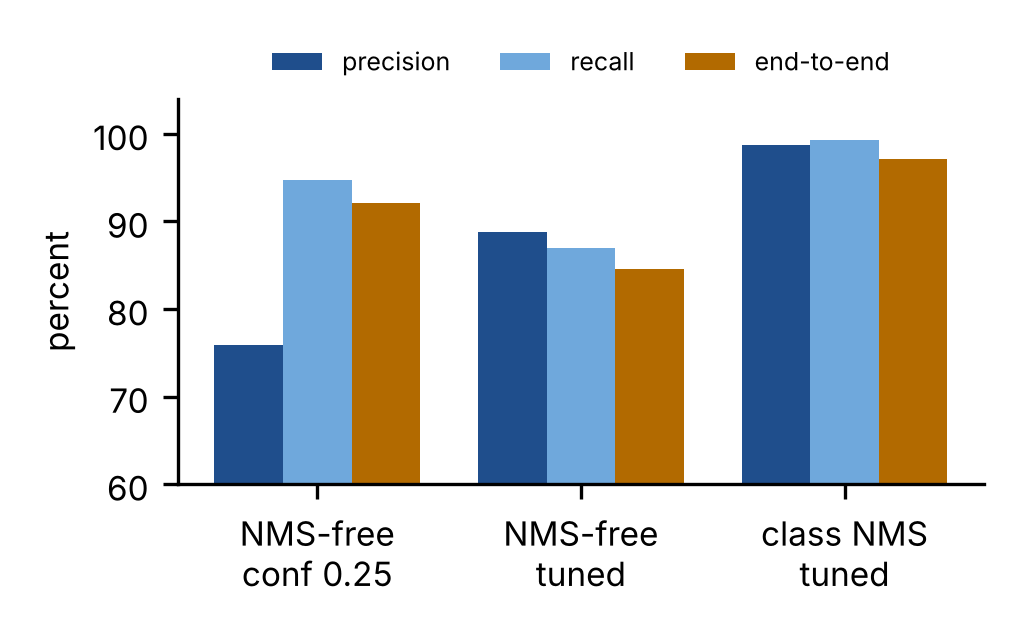
\includegraphics[width=0.95\columnwidth]{figures/variants.png}
\caption{Precision, recall, and end-to-end accuracy for the three operating points in Table~\ref{tab:main}. All values are percentages on one axis.}
\label{fig:variants}
\end{figure}

Three observations follow. First, adding class-wise suppression before OCR lifts precision from \valDefPrec\% to \valNmsPrec\% and end-to-end accuracy to \valNmsEndToEnd\%, and it also removes duplicate crops from the OCR stage. Second, tuning an NMS-free detector for validation F1 chose a high threshold (\valFreeConf{}) that traded away recall, and end-to-end accuracy fell to \valFreeEndToEnd\%, below the untuned default. F1 is not the end-to-end objective, and a threshold chosen for one can hurt the other. Third, the OCR stage is rarely the bottleneck. Among correctly localized text fields it was exact \valNmsOcrStage\% of the time with class NMS, and \valNmsOcrErrAllAccount{} \valNmsOcrErrCount{} errors were on account numbers: \valOcrErrExamples.

Fig.~\ref{fig:perclass} gives the per-class breakdown for the class-NMS variant. Account number is the weakest class, in both recall (\valRecAccountNumber\%) and OCR (\valOcrAccountNumber\%).

\begin{figure}[t]
\centering
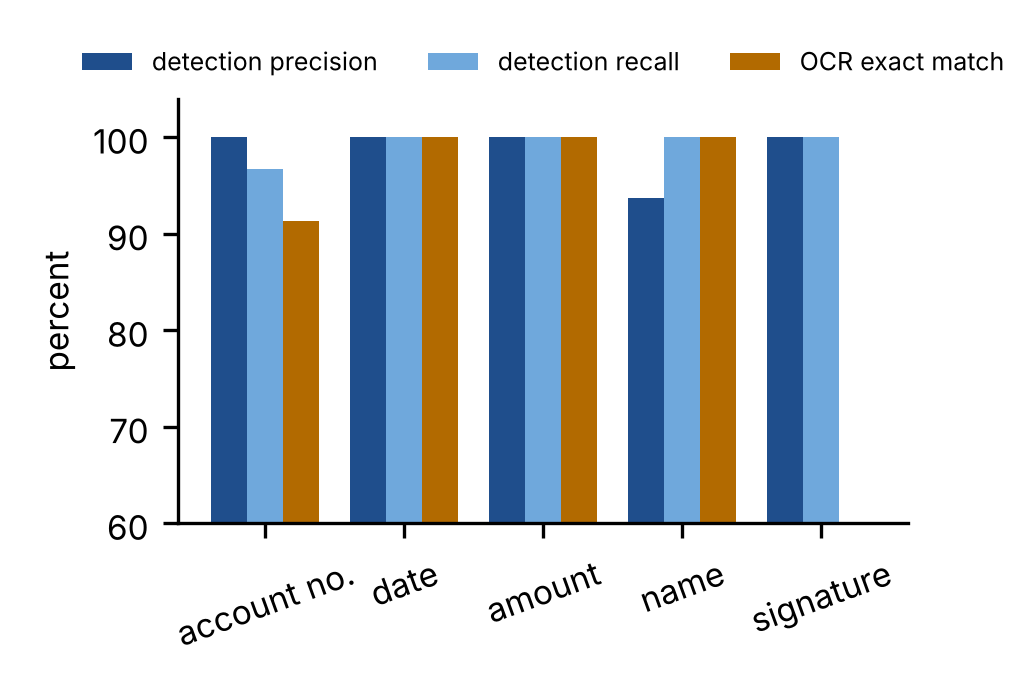
\includegraphics[width=0.95\columnwidth]{figures/per_class.png}
\caption{Per-class detection precision, recall, and OCR exact match for the class-NMS variant on the test split. The vertical axis starts at 60 percent. Signatures are detected but not read.}
\label{fig:perclass}
\end{figure}

\subsection{Comparison with full-page Tesseract}
Full-page Tesseract found \valBaseCapture\% of the 240 text strings somewhere on the page (95\% interval \valBaseLo{} to \valBaseHi), which is higher than the \valNmsEndToEnd\% end-to-end figure. We do not read this as a win for either side. On clean, large, printed text, page-level OCR reads almost every string, and our matching rule is lenient to it, because it never has to say which field a string belongs to. The detect-then-read pipeline pays for field attribution, which the baseline does not provide at all, and on this dataset it does not buy better reading. Whether detection helps on degraded scans, where page-level OCR loses accuracy \cite{thammarak2022,reisswig2019}, is the question this dataset cannot answer. Baseline cost was \valBaseSecPerDoc{} seconds per document on one process.

\subsection{Inference pattern}
Table~\ref{tab:pattern} and Fig.~\ref{fig:pattern} compare three ways of running the same detector over \valPatDocs{} documents in Spark on two partitions, with detection only. All three produced the same \valPatBoxes{} boxes, so they compute the same thing.

\begin{table}[t]
\centering
\caption{Inference pattern timing, mean and standard deviation of \valPatRepeats{} runs after one warm-up. CPU only, two cores.}
\label{tab:pattern}
\small
\begin{tabular}{@{}lccc@{}}
\toprule
Pattern & Seconds & Docs/s & Speedup \\
\midrule
Row-wise UDF, model per row & \valPatRowUdfSec{} $\pm$ \valPatRowUdfSd & \valPatRowUdfDps & 1.0 \\
\texttt{mapInPandas}, batch 1 & \valPatPartOneSec{} $\pm$ \valPatPartOneSd & \valPatPartOneDps & \valPatPartOneSpeedup \\
\texttt{mapInPandas}, batch 16 & \valPatPartSixteenSec{} $\pm$ \valPatPartSixteenSd & \valPatPartSixteenDps & \valPatPartSixteenSpeedup \\
\bottomrule
\end{tabular}
\end{table}

\begin{figure}[t]
\centering
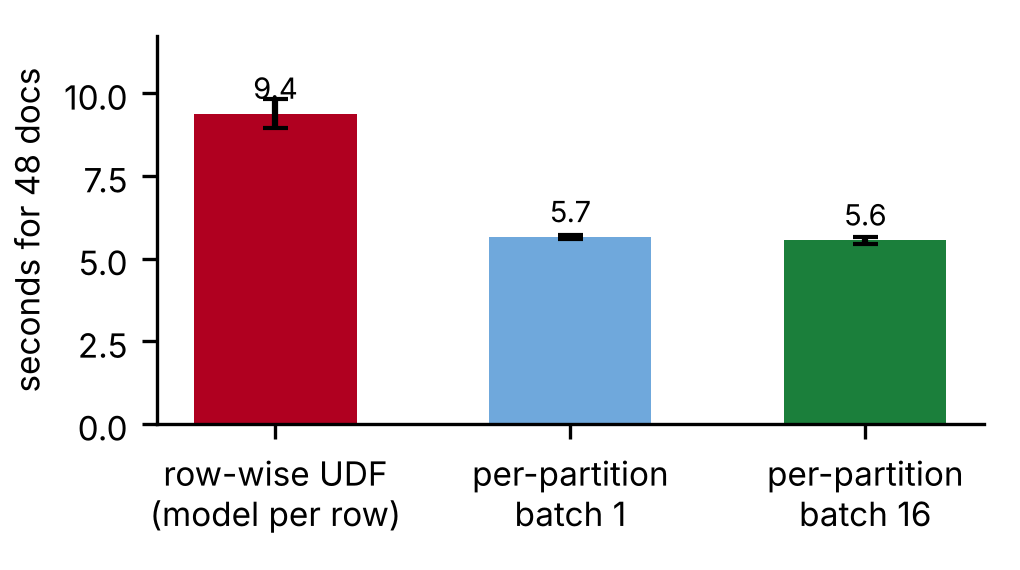
\includegraphics[width=0.95\columnwidth]{figures/pattern.png}
\caption{Wall time for \valPatDocs{} documents under three inference patterns. Error bars are one standard deviation over \valPatRepeats{} runs.}
\label{fig:pattern}
\end{figure}

Loading the model once per partition was \valPatPartSixteenSpeedup{} times faster than loading it per row. The implied cost of one model load is about \valPatLoadMs{} ms, which is small because the nano model is small, and the benefit would grow with a larger model and a CUDA context to initialize, which we did not measure. Arrow batch size 16 was not distinguishable from batch size 1 here (\valPatPartSixteenSec{} against \valPatPartOneSec{} seconds, within one standard deviation). The batching benefit that matters on a GPU is therefore untested by this experiment.

\subsection{Replication on a GPU}\label{sec:gpu}
We repeated the whole protocol once on a single NVIDIA \valGpuName{} GPU in Google Colab, with the same code, settings and Tesseract version. A recorded environment file shows that ONNX Runtime used the \valGpuProvider{} provider and that the \valGpuHashMatches{} test images were produced (SHA-256 prefix \valGpuTestHash), so Table~\ref{tab:gpu} compares the same documents. Training and the confidence sweep were run again, so the weights and the chosen thresholds differ from the CPU run. Spark still ran in local mode with two partitions, so this is a device check and does not exercise Spark GPU scheduling or the RAPIDS Accelerator.

\begin{table}[t]
\centering
\caption{Same protocol on CPU (two cores) and on one \valGpuName{} GPU. Both are single runs on the same 60 test documents.}
\label{tab:gpu}
\small
\begin{tabular}{@{}lcc@{}}
\toprule
 & CPU & \valGpuName{} \\
\midrule
Training time & \valTrainMinutes{} min & \valGpuTrainSeconds{} s \\
Val.\ mAP50 / mAP50-95 & \valMapFifty{} / \valMapFiftyNinetyFive & \valGpuMapFifty{} / \valGpuMapFiftyNinetyFive \\
Class NMS: P / R, \% & \valNmsPrec{} / \valNmsRec & \valGpuNmsPrec{} / \valGpuNmsRec \\
Class NMS: end to end, \% & \valNmsEndToEnd{} & \valGpuNmsEndToEnd{} \\
NMS-free, tuned: end to end, \% & \valFreeEndToEnd{} & \valGpuFreeEndToEnd{} \\
NMS-free, conf 0.25: end to end, \% & \valDefEndToEnd{} & \valGpuDefEndToEnd{} \\
Duplicates at conf 0.25 & \valDefDup{} & \valGpuDefDup{} \\
Row-wise UDF, s & \valPatRowUdfSec{} & \valGpuPatRowUdfSec{} \\
\texttt{mapInPandas}, batch 16, s & \valPatPartSixteenSec{} & \valGpuPatPartSixteenSec{} \\
Speedup, batch 16 & \valPatPartSixteenSpeedup{} & \valGpuPatPartSixteenSpeedup{} \\
\bottomrule
\end{tabular}
\end{table}

Detection and reading replicate: class-wise suppression again removed all duplicates and gave \valGpuNmsEndToEnd\% end-to-end accuracy (95\% interval \valGpuNmsEndToEndLo{} to \valGpuNmsEndToEndHi), and without it the end-to-end head again emitted duplicates (\valGpuDefDup{} at confidence 0.25). The ordering of the three variants is the same on both devices. Differences of a few points between the two columns cannot be separated into device effects and training variance, because each column is one training run on a 60-document test set, and we did not test them for significance. The per-partition speedup over the row-wise pattern held (\valGpuPatPartSixteenSpeedup{} times), but the GPU did not make this job faster. Every pattern was slower on the GPU than on the CPU, for example \valGpuPatPartSixteenSec{} against \valPatPartSixteenSec{} seconds at batch 16. A plausible reason is that a nano model on 640-pixel images is too small to repay device transfers and the initialization of two CUDA contexts, but we did not profile it. Training was the exception, and was much faster on the GPU. The GPU row therefore supports the same conclusions as the CPU run and shows no inference benefit for this small model.

An earlier run on the same GPU is worth recording. It gave only \valFallbackEndToEnd\% end-to-end accuracy because Colab lacked the DejaVu fonts, the generator silently used a different font, and the test images differed. Detection was unaffected (recall \valFallbackNmsRec\%), but reading was not. The released generator now stops with an error in that case. Reading accuracy on synthetic text is sensitive to the rendering environment, which is a further reason to treat all numbers here as properties of this dataset.

\subsection{Dataflow}
Fig.~\ref{fig:dataflow} contrasts the two inference patterns that Table~\ref{tab:pattern} measures.

\begin{figure}[t]
\centering
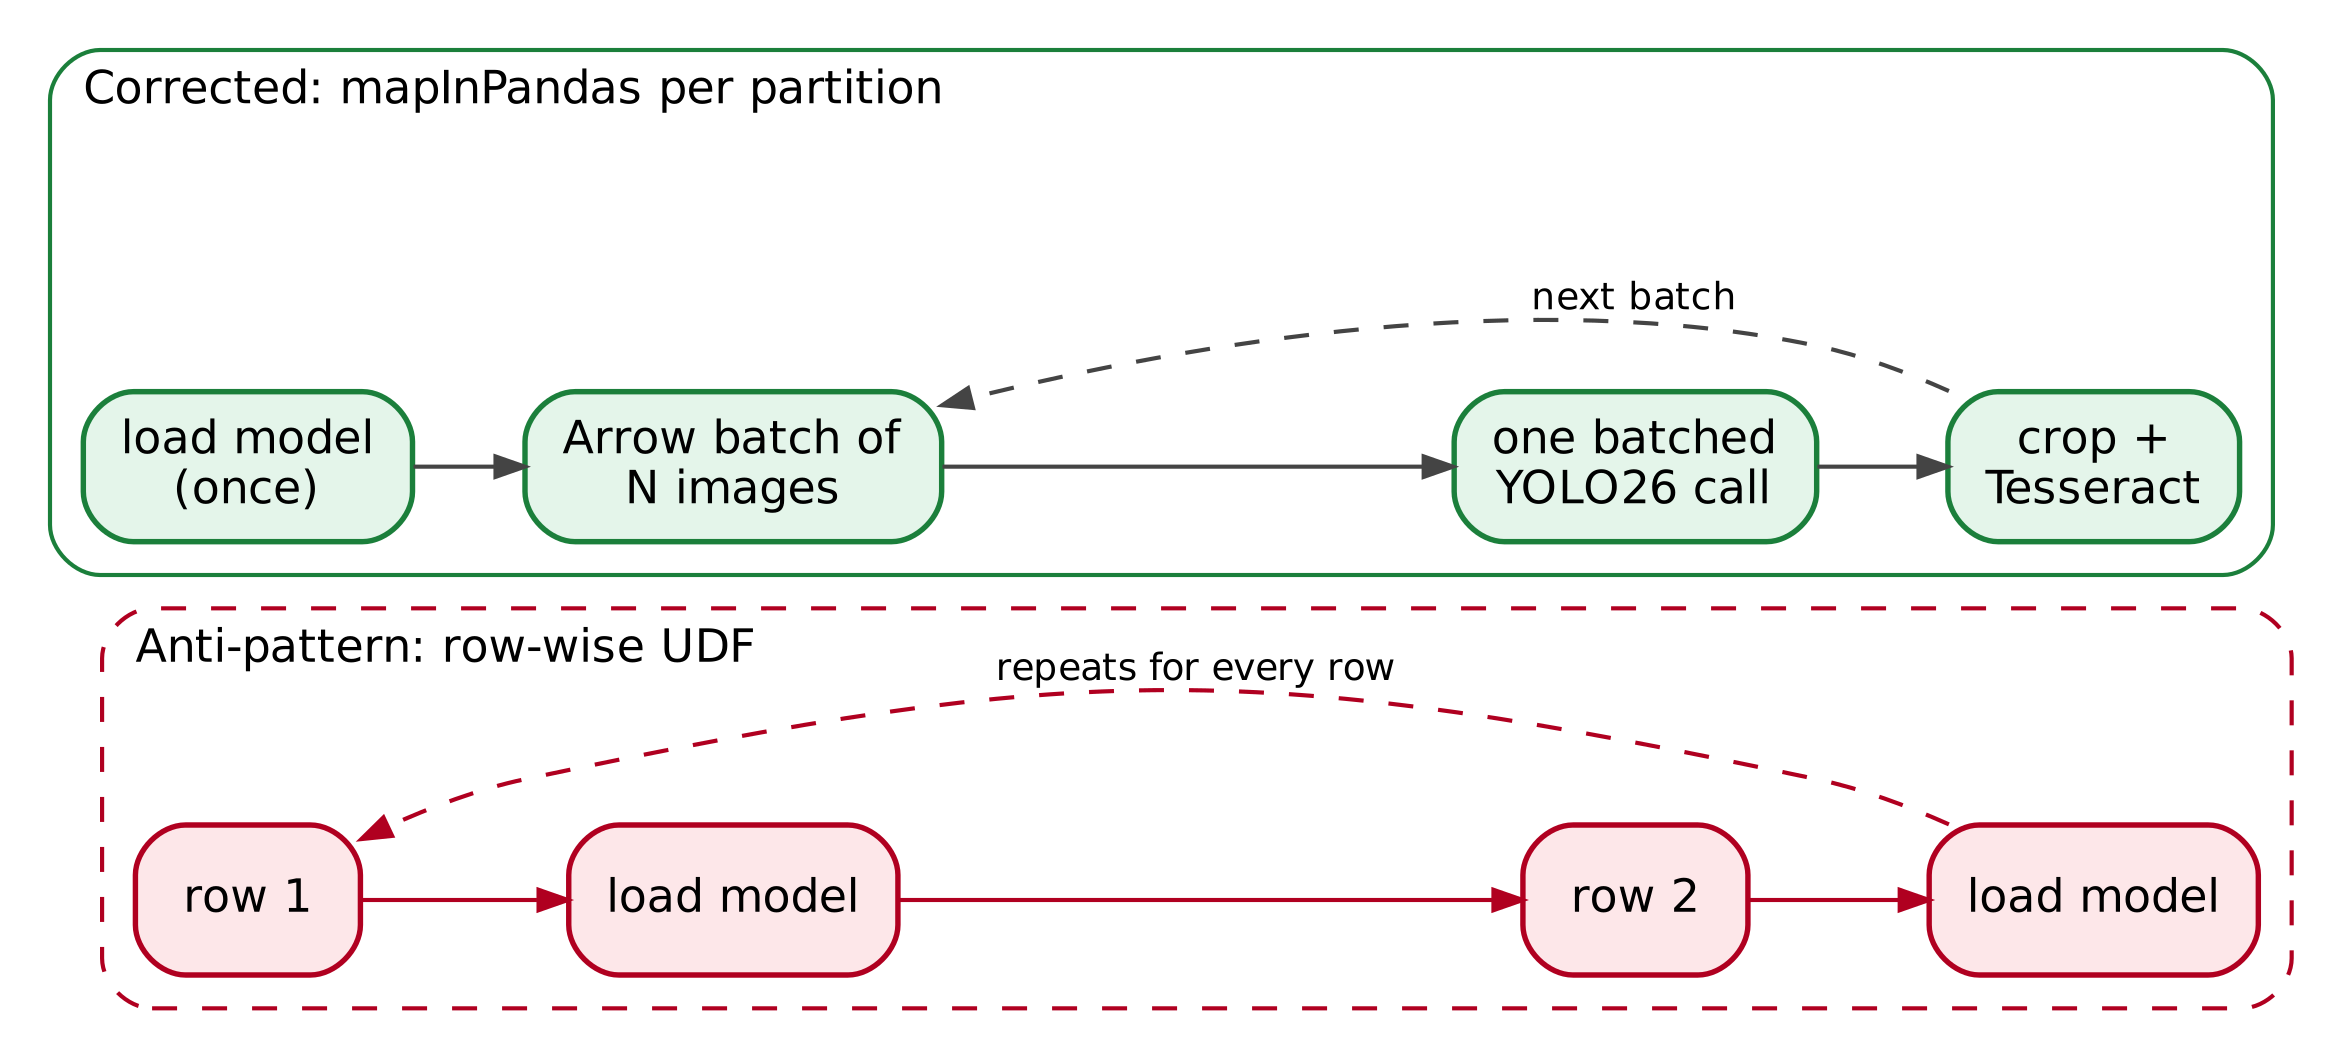
\includegraphics[width=0.95\columnwidth]{figures/dataflow.png}
\caption{Row-wise UDF versus partition-level \texttt{mapInPandas}. The first reloads the model for every row. The second loads it once per partition and then scores Arrow batches.}
\label{fig:dataflow}
\end{figure}

\section{Discussion and Limitations}
\textbf{What this supports.} The pipeline runs end to end under Spark, produces field-labeled text, and is reproducible from one repository. Loading the model per partition is faster than per row, and detection quality at a fixed threshold can differ sharply from the threshold-free mAP that training reports.

\textbf{What it does not support.} The dataset is synthetic, clean, and generated by one randomized form generator with three fonts and varied layout, noise and blur, so it is easy, and the high validation mAP reflects that. The results do not show that detection beats full-page OCR on real documents, and on this data it did not. There is one training run per device and a 60-document test split, so intervals are wide. The detector is the nano model. We ran the protocol on CPU and once on a single GPU in local Spark mode. Multi-node scaling, cluster start-up, cost, Spark GPU scheduling with the RAPIDS Accelerator, and Amazon Textract were not measured, and the cluster GPU configuration in the released code is untested. Stronger baselines, such as LayoutLMv3 \cite{huang2022layoutlmv3}, Donut \cite{kim2022donut}, and other open OCR engines, were not run.

\textbf{Cold start.} The batch design assumes cluster start-up cost is amortized over a queue of documents. It is a poor fit for sub-second interactive requests, for which a warm cluster or a dedicated model server is the better choice.

\textbf{Next steps.} The most informative next experiment is the same protocol on real, degraded scans with field-level labels, where the comparison with page-level OCR could go either way, followed by the GPU path on EMR with a larger model, where device use may matter more than it did here.

\section{Ethical Considerations}
Checks and identification documents contain sensitive personal data. All data here is synthetic. Any use of real documents should follow the institution\textquotesingle{}s data-governance process and data-minimization principles such as those in the GDPR \cite{gdpr}, with encryption at rest, separate access scopes for raw images and structured output, and human review for low-confidence detections rather than automated decisions. Synthetic data from one generator does not establish fair performance across banks, regions, and languages, and that should be tested directly.

\section{Conclusion}
We built and released a Spark pipeline that detects financial form fields with YOLO26 and reads each with Tesseract, and we checked it by running it. The integration defects were real and are cataloged. On clean synthetic forms the pipeline reaches \valNmsEndToEnd\% end-to-end field accuracy with class-wise suppression, the end-to-end head emitted duplicates without it, and full-page OCR read the same strings at least as well, without saying which field each belonged to. Loading the model once per partition was \valPatPartSixteenSpeedup{} times faster than per row on CPU, and \valGpuPatPartSixteenSpeedup{} times on one GPU, where the nano model gained no inference speed. Real scanned documents, cluster-scale GPU execution, and stronger baselines are the open questions, and the released code is meant to make those experiments cheap to run.
